\ifthenelse{\equal{\Langue}{FR}}{
\chapter{Alimentation à découpage Flyback pour chargeur de batterie}
}{
\chapter{Flyback converter for battery charger}
}

\ifthenelse{\equal{\Langue}{FR}}{
Il s'agit d'utiliser le montage de la figure suivante pour réaliser un chargeur de batterie de tension nominale 24V.
}{
The goal is to use the circuit shown in the following figure to create a 24V battery charger.
}

\begin{figure}[h]
\centering
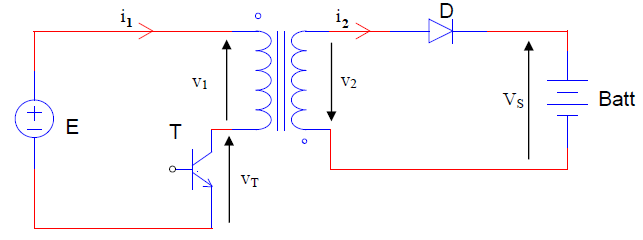
\includegraphics[width=0.8\linewidth]{TD_Flyback/fig/FlybackBatterie.png}
\end{figure}

\ifthenelse{\equal{\Langue}{FR}}{
On note $n_1$ et $n_2$ les nombres de spires respectifs au primaire et au secondaire, le rapport de transformation étant
noté $m$, l'inductance magnétisante primaire sera quant à elle notée $L_1$, la fréquence de découpage $f$, le rapport
cyclique $\alpha$.

La batterie initialement déchargée a une tension à ses bornes $V_{S0} = 20V$. On arrêtera sa charge lorsque la tension
à ses bornes atteindra $V_{S1} = 26 V$. Néanmoins, dans toute l'étude, cette tension batterie, notée $V_S$, sera supposée
constante à l'échelle de temps du découpage.

En débutant la charge de la batterie, on suppose que l'alimentation fonctionne en régime critique avec un rapport cyclique $\alpha_0$, le courant moyen dans la batterie est alors égal à $I_{S0}$.

\vspace{0.25cm}
Valeurs numériques: $E = 300V$; $f = 20 kHz$; $\alpha_0 = 0.5$; $I_{S0} = 10 A$.
}{
Let $n_1$ and $n_2$ be the respective numbers of turns in the primary and secondary windings, with the transformation ratio denoted as $m$. The primary magnetizing inductance is denoted as $L_1$, the switching frequency as $f$, and the duty cycle as $\alpha$.

The initially discharged battery has a voltage of $V_{S0} = 20V$ across its terminals. The charging process will be stopped when the voltage across the terminals reaches $V_{S1} = 26V$. However, throughout the analysis, this battery voltage, denoted as $V_S$, will be assumed to be constant on the timescale of the switching.

At the beginning of the battery charging process, it is assumed that the power supply operates in critical mode with a duty cycle of $\alpha_0$, and the average current in the battery is $I_{S0}$.

\vspace{0.25cm}
Numerical values: $E = 300V$; $f = 20 kHz$; $\alpha_0 = 0.5$; $I_{S0} = 10 A$.
}

\begin{enumerate}
%%%%%% Partie 1 %%%%%%%

\ifthenelse{\equal{\Langue}{FR}}{
\item \textbf{Début de charge}
}{
\item \textbf{Start of charging}
}
\begin{enumerate}


\ifthenelse{\equal{\Langue}{FR}}{
\item Donner l'expression du théorème d'Hopkinson liant $n_1$, $i_1$, $n_2$ et $i_2$ à $R$ réluctance de la ferrite (inverse de l'inductance spécifique $A_L$),  et $\varphi$ flux élémentaire dans celle-ci.
}{
\item Provide the expression of Hopkinson's theorem relating $n_1$, $i_1$, $n_2$, $i_2$, and $R$ (reluctance of the ferrite core, inverse of the specific inductance $A_L$), and $\varphi$ (elementary flux in the core).
}

\ifthenelse{\equal{\SuCorr}{CO}}{
$n_1 i_1 + n_2 i_2 = R \varphi$
}

\ifthenelse{\equal{\Langue}{FR}}{
\item Représenter sur une période de découpage l'allure des signaux $i_1$, $i_2$, $\varphi$, $v_T$ et $v_1$.
}{
\item Plot the waveforms of $i_1$, $i_2$, $\varphi$, $v_T$, and $v_1$ over one switching period.
}

\ifthenelse{\equal{\SuCorr}{CO}}{
\begin{itemize}
    \item \underline{$0 < t < \alpha T$}: T ``\ifthenelse{\equal{\Langue}{FR}}{fermé}{closed}'' $\rightarrow v_T = 0$; $v_1 = E$; $v_2 = \dfrac{n_2}{n_1} E > 0$
    
    $v_D=-v_2 - V_S < 0$ $\rightarrow$ D ``\ifthenelse{\equal{\Langue}{FR}}{bloquée}{reverse}'' $\rightarrow i_2 = 0$;
    
    $v_1 = E = L_1 \dfrac{di_1}{dt}$ \ifthenelse{\equal{\Langue}{FR}}{et régime critique}{and boundary mode} $\rightarrow \varphi(t=0)=0$ $\rightarrow$ $i_1(t=0) = 0$

    $i_1(t)=\dfrac{E}{L_1} t$; $v_1=n_1 \dfrac{d\varphi}{dt}$ $\rightarrow$ $\varphi(t)=\dfrac{E}{n_1} t$
    \item \underline{$\alpha T < t < T$}: T ``\ifthenelse{\equal{\Langue}{FR}}{ouvert}{open}'' $\rightarrow i_1 = 0$
    
    \ifthenelse{\equal{\Langue}{FR}}{Continuité du flux}{Flux continuity} $\rightarrow$ $i_2(\alpha T^+)>0$ $\rightarrow$ D ``\ifthenelse{\equal{\Langue}{FR}}{passante}{forward}'' $\rightarrow v_2 = -V_S$; $v_1 = -\dfrac{n_1}{n_2} V_S$
    
    $v_T = E - v_1 = E + \dfrac{n_1}{n_2} V_S$

    $v_2=n_2 \dfrac{d\varphi}{dt}$ $\rightarrow$ $\varphi(t)=-\dfrac{V_S}{n_2} (t-\alpha T)$ \hspace{0.5cm} ($\varphi(\alpha T)=0$ \ifthenelse{\equal{\Langue}{FR}}{car régime critique}{because boundary mode})
\end{itemize}

\begin{figure}[H]
\centering
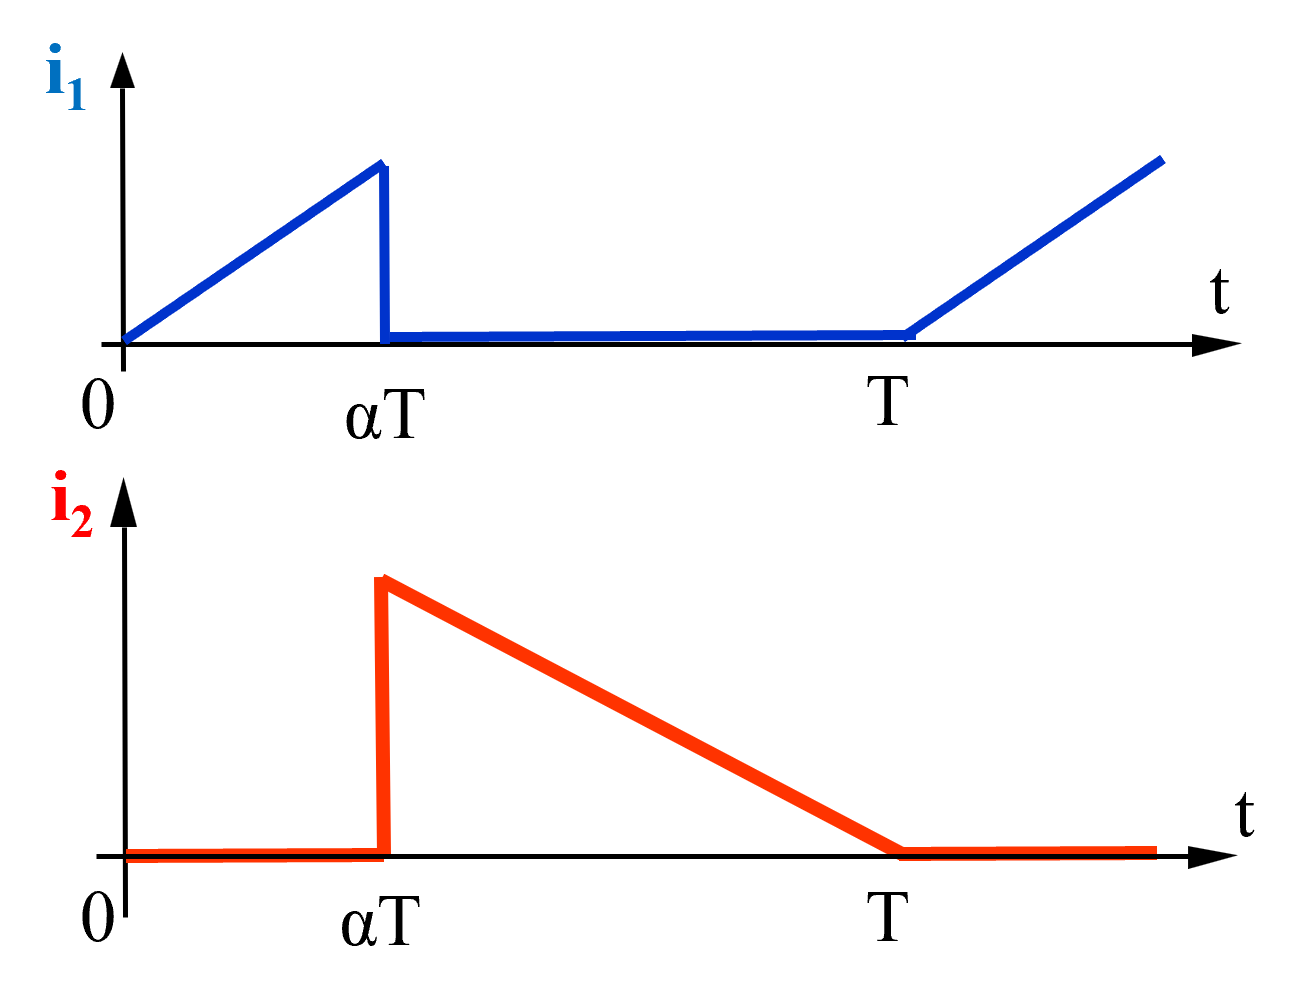
\includegraphics[width=0.45\linewidth]{TD_Flyback/fig/Flyback_Q12_I12.png}
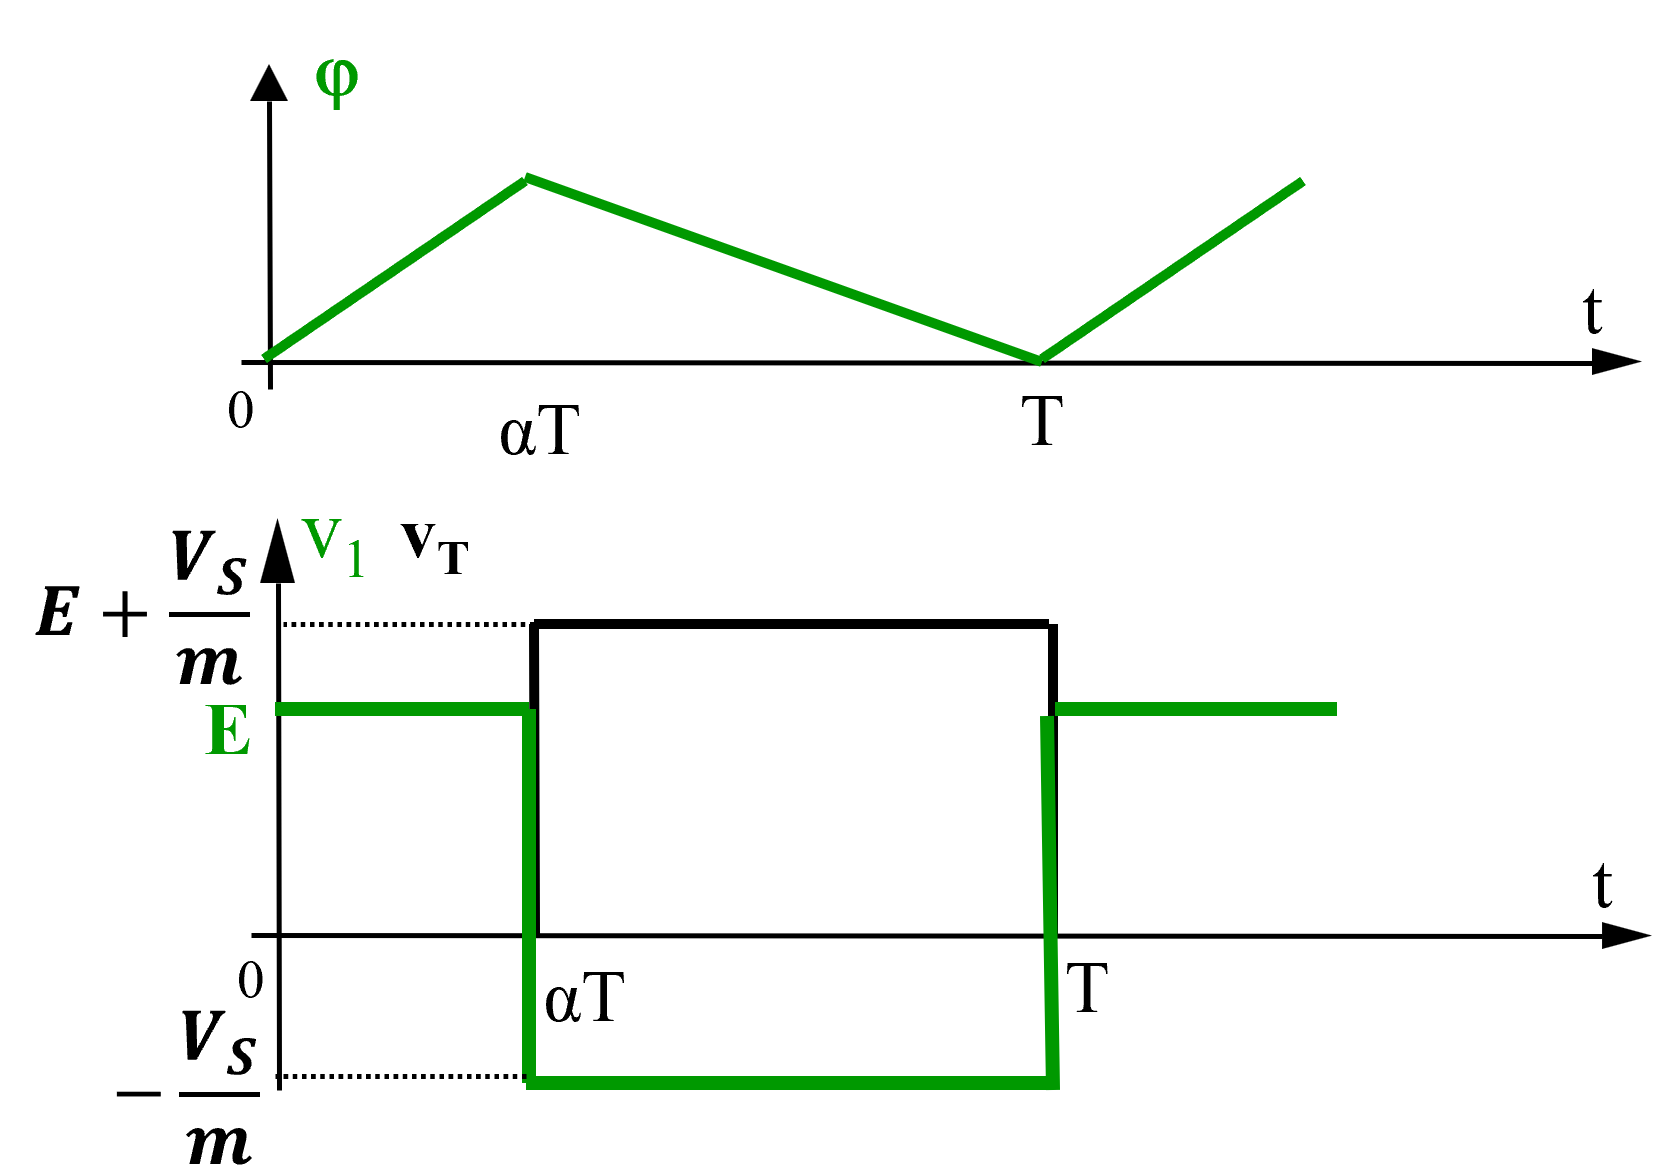
\includegraphics[width=0.45\linewidth]{TD_Flyback/fig/Flyback_Q12_phi_v12.png}

\end{figure}
}

\ifthenelse{\equal{\Langue}{FR}}{
\item En déduire l'expression de la tension de sortie $V_S$ en fonction de $E$, $m$ et $\alpha_0$. En déduire la valeur numérique de $m$.
}{
\item Deduce the expression of the output voltage $V_S$ in terms of $E$, $m$, and $\alpha_0$. Calculate the numerical value of $m$.
}

\ifthenelse{\equal{\SuCorr}{CO}}{
$<v_1> = 0$ $\rightarrow$ $E \alpha - \dfrac{n_1}{n_2} V_S (1-\alpha) = 0$ $\rightarrow$ $V_S = m\dfrac{\alpha}{1-\alpha} E$

%%%%%%%%%%%%%%%%%%%%%%%%%%%%% TO CONTINUE %%%%%%%%%%%%%%%%%%%%%%%%%%%%%

}

\ifthenelse{\equal{\Langue}{FR}}{
\item Déterminer l'expression du courant moyen de sortie noté $I_{S0}$ en fonction de $L_1$, $\alpha_0$, $m$, $E$ et $f$. En
déduire la valeur numérique de l'inductance $L_1$.
}{
\item Determine the expression of the average output current $I_{S0}$ in terms of $L_1$, $\alpha_0$, $m$, $E$, and $f$. Calculate the numerical value of $L_1$.
}

\ifthenelse{\equal{\SuCorr}{CO}}{
$I_{S0} = <i_2> = \dfrac{1}{T} \int_{0}^{T} i_2(t) dt = \dfrac{1}{T} \int_{\alpha T}^{T} i_2(t) dt$
}

\ifthenelse{\equal{\Langue}{FR}}{
\item Calculer de deux façons différentes l'énergie $W_D$ fournie par cycle de découpage à la batterie.
}{
\item Calculate the energy $W_D$ delivered to the battery per switching cycle using two different methods.
}

\ifthenelse{\equal{\SuCorr}{CO}}{

}

\ifthenelse{\equal{\Langue}{FR}}{
\item Calculer numériquement cette énergie $W_D$ et en déduire le temps de charge à courant constant pour une batterie de `` capacité'' 25 Ah.
}{
\item Calculate the numerical value of this energy $W_D$ and determine the charging time at constant current for a battery with a ``capacity'' of 25 Ah.
}

\ifthenelse{\equal{\SuCorr}{CO}}{

}

\end{enumerate}


%%%%%% Partie 2 %%%%%%%
\ifthenelse{\equal{\Langue}{FR}}{
\item \textbf{Fin de charge}

Lors de la charge, la tension de sortie évolue lentement de $V_{S0}$ à $V_{S1}$, le rapport cyclique étant maintenu à $\alpha_0$.
\begin{enumerate}
\item Comment le régime de conduction de l'alimentation a-t-il été modifié?
\item  Représenter sur une période de découpage l'allure des signaux $ i_1$, $i_2$, $v_T$ et $v_1$.
\item Quelle est la durée de conduction de la diode D\@?
\item Que vaut maintenant l'énergie transférée par cycle? En déduire le courant moyen $I_S$ fourni à la batterie.
\item Quelle valeur $\alpha_1$ faudrait-il donner au rapport cyclique pour fournir ensuite un courant moyen de charge de batterie 
$I_{S1} = I_{S0}/10$?
\end{enumerate}
}{
\item \textbf{End of charging}

During the charging process, the output voltage slowly increases from $V_{S0}$ to $V_{S1}$ while maintaining the duty cycle at $\alpha_0$.
\begin{enumerate}
\item How has the conduction mode of the power supply been modified?
\item Plot the waveforms of $i_1$, $i_2$, $v_T$, and $v_1$ over one switching period.
\item What is the conduction time of the diode D\@?
\item What is the energy transferred per cycle now? Determine the average current $I_S$ supplied to the battery.
\item What value $\alpha_1$ should be given to the duty cycle to subsequently provide an average charging current of $I_{S1} = I_{S0}/10$?
\end{enumerate}
}

%%%%%% Partie 3 %%%%%%%
\ifthenelse{\equal{\Langue}{FR}}{
\item \textbf{Limite de saturation}

On se place en régime critique (début de charge)

\begin{enumerate}
\item Déterminer l'expression de l'induction maximale dans la ferrite en fonction de E, $\alpha$, T, $n_1$ et $A_e$, surface effective de cette ferrite.
\item En déduire l'expression de la valeur minimale $A_{e\ \min}$ de cette ferrite pour empêcher toute saturation du matériau: on notera pour cela $B_{sat}$ la valeur de l'induction au voisinage de la saturation.
\end{enumerate}
}{
\item \textbf{Saturation limit}

We are in the critical mode (start of charging).

\begin{enumerate}
\item Determine the expression of the maximum magnetic induction in the ferrite core in terms of $E$, $\alpha$, $T$, $n_1$, and $A_e$ (effective area of the core).
\item Deduce the expression of the minimum value $A_{e\ \min}$ of the core area to prevent any saturation of the material. For this purpose, let $B_{sat}$ be the induction value near saturation.
\end{enumerate}
}

%%%%%% Partie 4 %%%%%%%
\ifthenelse{\equal{\Langue}{FR}}{
\item \textbf{Surface de la fenêtre de bobinage}

On reste en régime critique (début de charge)

\begin{enumerate}
\item En utilisant les résultats de la première partie, déterminer la valeur efficace $I_{1\ eff}$ du courant dans le transistor en fonction du courant de sortie $I_s$, de $m$ et $\alpha$.
\item Faire de même pour exprimer la valeur efficace $I_{2\ eff}$ du courant secondaire en fonction de $I_s$ et $\alpha$.
\item La densité de courant choisie pour ces deux bobinages réalisés en fil de cuivre est $\delta$. Déterminer l'expression de la surface totale de cuivre, notée $S_{T\ Cu}$, en fonction de $I_s$, $\delta$, $n_2$ et $\alpha$. Comparer les surfaces de cuivre primaire et secondaire.
\item En déduire la surface minimale de la fenêtre de bobinage, notée $S_B$, si l'on choisit un coefficient de bobinage $k_B$ ($S_{T\ Cu} = k_B.S_B$).
\end{enumerate}
}{
\item \textbf{Winding window area}

We are still in the critical mode (start of charging).

\begin{enumerate}
\item Using the results from the first part, determine the RMS value of the current in the transistor $I_{1\ eff}$ in terms of the output current $I_s$, $m$, and $\alpha$.
\item Similarly, express the RMS value  of the secondary current $I_{2\ eff}$ in terms of $I_s$ and $\alpha$.
\item The chosen current density for both windings made of copper wire is $\delta$. Determine the expression of the total copper area, denoted as $S_{T\ Cu}$, in terms of $I_s$, $\delta$, $n_2$, and $\alpha$. Compare the primary and secondary copper areas.
\item Deduce the minimum winding window area, denoted as $S_B$, if a winding coefficient $k_B$ is chosen ($S_{T\ Cu} = k_B.S_B$).
\end{enumerate}
}

%%%%%% Partie 5 %%%%%%%
\ifthenelse{\equal{\Langue}{FR}}{
\item \textbf{Choix du noyau magnétique}

\begin{enumerate}
\item A partir des résultats des questions précédentes, déterminer l'inégalité que doit vérifier le produit $A_e.S_B$ de cette alimentation en fonction de $B_{sat}$, $P_s$, $T$, $k_B$, $\delta$ et $\alpha$.
\item Calculer cette valeur minimale en $mm^4$ pour les valeurs numériques suivantes:

\begin{center}
$P_s = 200 W$; $\alpha = 0.5$; $k_B = 0.5$; $B_{sat} = 0.4 T$; $\delta = 5 A.mm^{-2}$; $f = 20 kHz$.
\end{center}

\newpage
\item Choisir un noyau parmi la liste suivante pour laquelle on donne les valeurs de $A_e$, $S_B$ et $A_L$ fournies par le constructeur (on rappelle que $A_L$ désigne l'inductance spécifique pour une spire), tous ces noyaux étant réalisés avec le même matériau $N41$.
}{
\item \textbf{Choice of magnetic core}

\begin{enumerate}
\item Based on the previous questions, determine the inequality that the product $A_e.S_B$ of this power supply must satisfy in terms of $B_{sat}$, $P_s$, $T$, $k_B$, $\delta$, and $\alpha$.
\item Calculate the minimum value of this product in $mm^4$ for the following numerical values:

\begin{center}
$P_s = 200 W$; $\alpha = 0.5$; $k_B = 0.5$; $B_{sat} = 0.4 T$; $\delta = 5 A.mm^{-2}$; $f = 20 kHz$.
\end{center}

\item Choose a core from the following list, for which the manufacturer provides the values of $A_e$, $S_B$, and $A_L$ (specific inductance) without air gap, as well as $A_L$ with a 0.5 mm air gap. Note that all these cores are made of the same material, $N41$.
}

\vspace{1mm}
\begin{tabular}{|c|c|c|c|c|}
\hline
\multirow{2}*{Core} & \multirow{2}*{$A_e\ (mm^2)$} & \multirow{2}*{$S_B \ (mm^2)$} & $A_L$ without air gap & $A_L$ 0.5 mm air gap\\
& & & (nH) & (nH)\\
\hline
RM6 & 31 & 32 & 3100 & ---\\
\hline
RM8 & 55 & 57 & 4100 & 160\\
\hline
RM10 & 90 & 93 & 5500 & 250\\
\hline
RM12 & 125 & 128 & 6000 & 300 \\
\hline
RM14 & 170 & 176 & 6800 & 400 \\
\hline
\end{tabular}

\vspace{1mm}

\ifthenelse{\equal{\Langue}{FR}}{
\item Pour ce choix de noyau, déterminer alors les nombres de spires minimaux $n_1$ et $n_2$ pour limiter l'induction maximale dans la ferrite à $B_{sat}$. Pour ces calculs, on choisira  ``au mieux'' ces valeurs de nombres de spires pour les valeurs numériques ci-dessus.

\item Un entrefer sera-t-il nécessaire afin d'obtenir l'inductance $L_1$ souhaitée?
\end{enumerate}
}{
\item For this choice of core, determine the minimum numbers of turns $n_1$ and $n_2$ to limit the maximum induction in the ferrite core to $B_{sat}$. For these calculations, choose the values of the numbers of turns that are ``optimal'' for the given numerical values.

\item Will an air gap be necessary to achieve the desired inductance $L_1$?
\end{enumerate}
}



\begin{figure}[h]
\centering
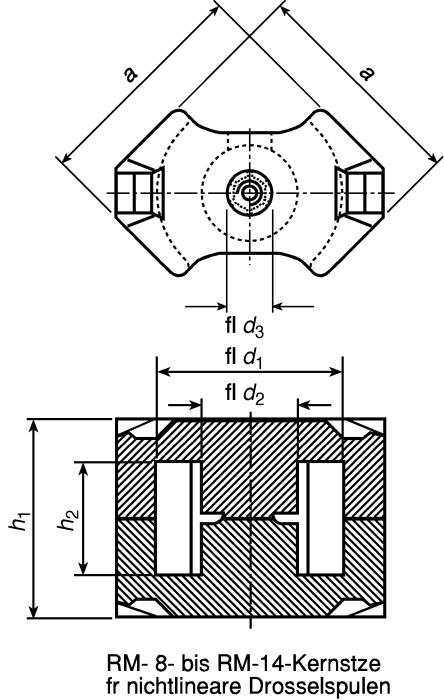
\includegraphics[width=0.5\linewidth]{TD_Flyback/fig/noyau.png}
\end{figure}

\end{enumerate}